\documentclass{article}
\usepackage{graphicx}
\usepackage{amsmath}
\usepackage{hyperref}
\usepackage{cleveref}

\graphicspath{{figs/}}

\begin{document}

Saturating Activator

\begin{align}
    a'[t] &= \frac{ S^n }{ Km^n + S^n } - a(t) \\
    i'(t) &= \alpha * ( S - i(t)) \\
    r'(t) &= \beta * ( a(t) ( R_{tot} - r(t) ) - i(t) r(t) )
\end{align}

\begin{itemize}
    \item for $Km \ll S$, it's the original LEGI model
    \item for $Km \approx S$ and $n=1$, saturated activator
    \item for $Km \approx S$ and $n>1$, sigmoidal activator
\end{itemize}

\begin{figure}
    \centering
    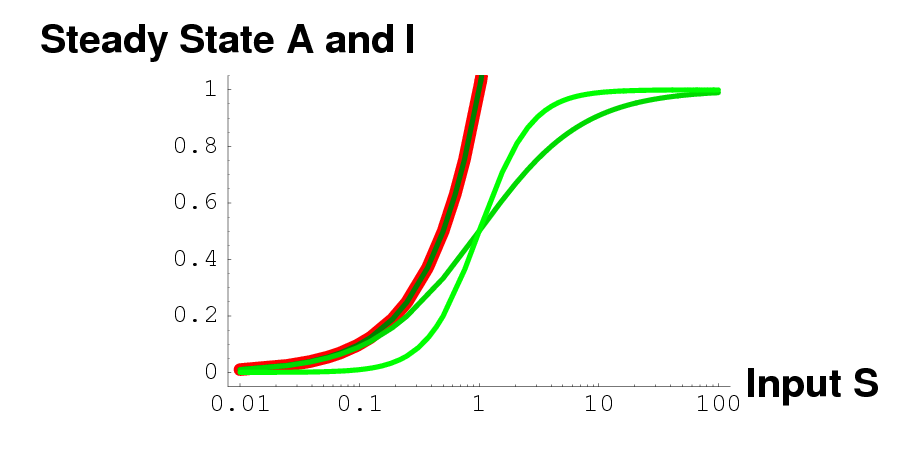
\includegraphics[width=0.9\textwidth]{ssAIR.png}
    \caption{Steady state activator, nonconserved (dark green),
        saturating (green), sigmoidal (lime) and steady state,
        nonconserved inhibitor (red). \label{fig:metric}}
\end{figure}


\begin{figure}
    \centering
    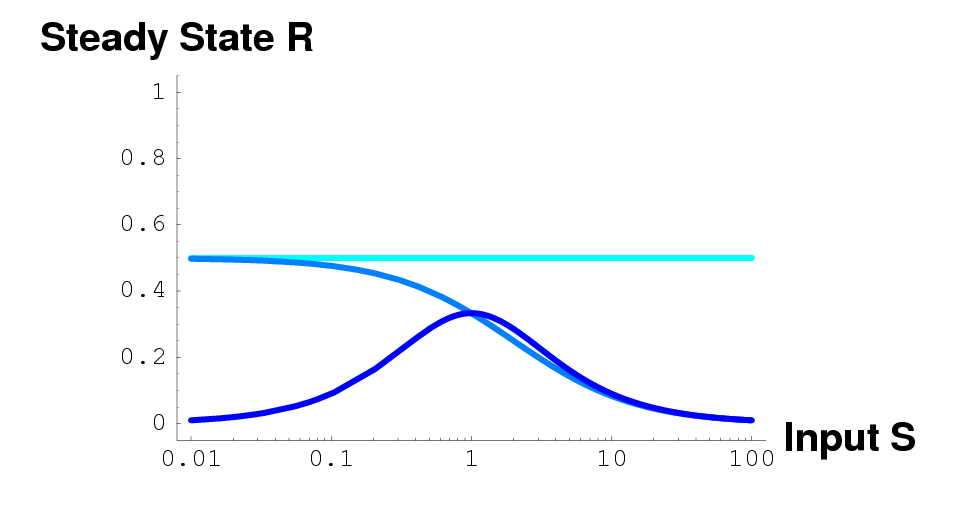
\includegraphics[width=0.9\textwidth]{ssR.png}
    \caption{Steady state response for LEGI (cyan),
        saturating activator (blue), sigmoidal activator (navy)
        \label{fig:metric}}
\end{figure}

\begin{figure}
    \centering
    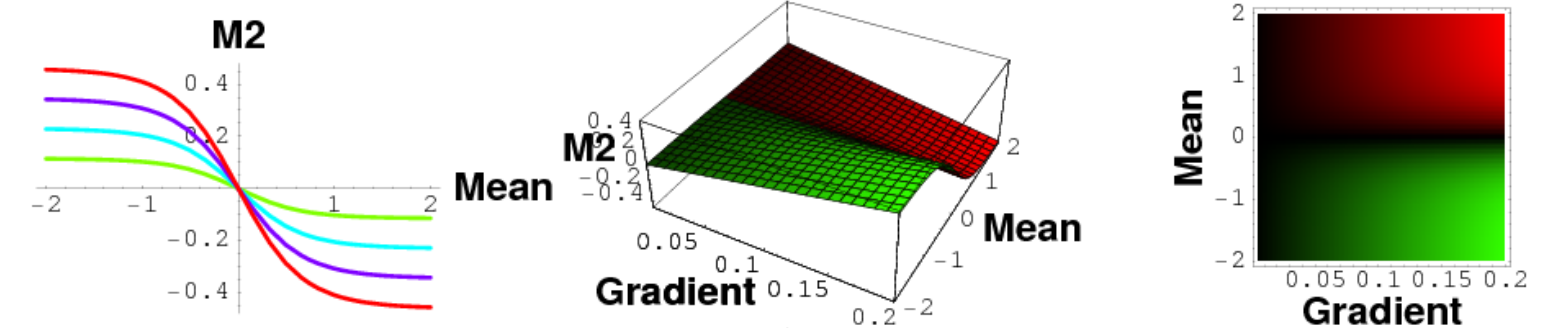
\includegraphics[width=0.9\textwidth]{metric.png}
    \caption{Metric \label{fig:metric}}
\end{figure}

\begin{figure}
    \centering
    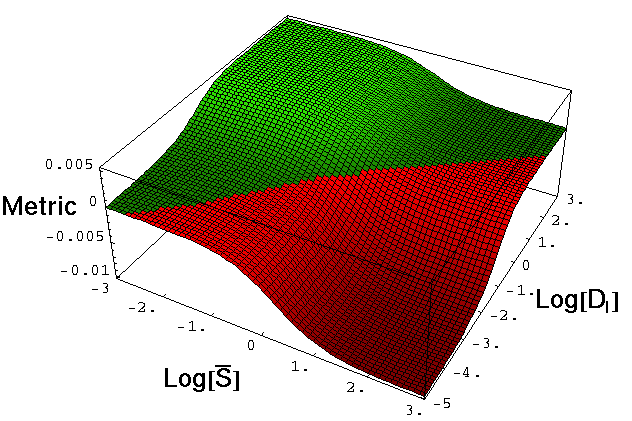
\includegraphics[width=0.9\textwidth]{MetricVsAvgVsDi.png}
    \caption{Metric \label{fig:metric}}
\end{figure}


the "stopping point" - point in the gradient when attraction becomes repulsion

neuronal migration based on a local model

Mechanical model
\cref{fig:tension_fig}
\begin{figure}
    \centering
    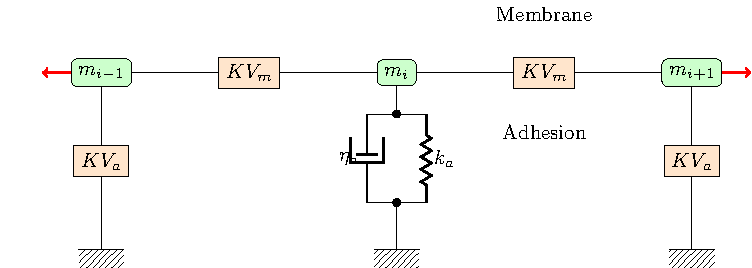
\includegraphics[width=0.9\textwidth]{./tension_fig.pdf}
    \caption{Membrane model \label{fig:tension_fig}}
\end{figure}

Kelvin-Voigt elements


\begin{align}
    s_i     &= L * \frac{ i-1 }{ n-1 }  \\
    x_i(0)  &= s_i \\
    x'_i(0) &= 0 \\
    m * x''_i(t) &= k_a (s_i - x_i(t)) - \eta_m * x_i'(t)  \\
                 &\phantom{{}=}+ Fm_i(t) + Fm_{i-1}(t) \notag \\
    Fm_i(t) &= k_m \left( \frac{ x_{i+1}(t) - x_i(t) }{ dL } - 1 \right)  \\
            &\phantom{{}=} - \eta_m \left(x_i(t) - x_{i+1}(t) \right) \notag
\end{align}

\iffalse

Steady-state

\begin{align}
   a_{ss} &= A_{tot} * \frac{ S }{ 1 + S } \\
   i_{ss} &= S \\
   r_{ss} &= A_{tot} * \frac{ R_{tot} }{ 1 + S + A_{tot} } 
\end{align}

\begin{itemize}
    \item noisy gradients? 
    \item inputs varying in time
    \item inputs varying in space
\end{itemize}

\fi

\end{document}

